\documentclass[blue]{beamer}
\usepackage{beamerthemeFrankfurt} 
\usecolortheme{rose}
\usepackage{amsmath}
\usepackage{amssymb}
%\usepackage{cite} % never use with beamer 
\usepackage{hyperref}
\usepackage{latexsym}
\usepackage{graphicx}
\usepackage{multirow}
\usepackage[export]{adjustbox}
\makeatletter
\newcommand{\removelatexerror}{\let\@latex@error\@gobble}
\makeatother
\usepackage{url}
\newtheorem{assumption}{Assumption}
\usepackage{setspace}
\setbeamertemplate{itemize/enumerate body begin}{\small}
\usepackage{tabulary}
\usepackage{subfig}
\usepackage{listings}
\lstset{language=Java,
                basicstyle=\footnotesize\ttfamily,
                keywordstyle=\footnotesize\color{blue}\ttfamily,
}

\usepackage[linesnumbered,ruled]{algorithm2e} 
%\usepackage{algpseudocode,algorithm,algorithmicx}
\setbeamercolor{title}{fg=red!80!black,bg=red!20!white}
 %   \setbeamerfont{block title}{size=\scriptsize} change block title font size
%\setbeamerfont{title}{shape=\itshape,family=\rmfamily}
%\usetheme{Warsaw} % brings shadowness
\usefonttheme{professionalfonts} % font theme
\newtheorem{answeredquestions}[theorem]{Answered Questions}
\usepackage[figuresright]{rotating}
\usepackage{subfig}
\makeatletter
\let\@@magyar@captionfix\relax
\makeatother
\usepackage[
  separate-uncertainty = true,
  multi-part-units = repeat
]{siunitx}
\graphicspath{{images/}{use/}{infersent/}}
%\usefonttheme[onlysmall]{structurebold} %%%small fonts in the navigation bars are a bit hard

\title{Data Stream Mining}
\author[Chandresh]{Chandresh Kumar Maurya, Assistant Professor}

\author[Peter]{P\'eter Kiss, Teaching Assistant}
\institute{E\"otv\"os Lor\'and University, Budapest, Hungary}
\begin{document}
\maketitle



%====================================================


\section{Intoduction}

\begin{frame}{Data Stream }
\begin{block}{Definition}
A data stream is an ordered (not necessarily always) and potentially infinite sequence of data points.
\begin{center}
    $x_1,x_2, x_3,\ldots,$
\end{center}
where $x_i$s are tuples constituted of numbers, words, sequences, etc.
\end{block}

\end{frame}


\begin{frame}{DSMS}
\begin{block}{Data Stream Management System (DSMS)}
\begin{itemize}
    \item Software system to manage continuous data streams. 
 
\item Similar to a database management system (DBMS), which is, however, designed for static data in conventional databases.
 
\item offers a flexible query processing so that the information needed can be expressed using queries.

\item  DSMS executes a continuous query that is not only performed once, but is permanently installed. That is, the query is continuously executed until it is explicitly uninstalled. 

\item most DSMS are data-driven, a continuous query produces new results as long as new data arrive at the system. 
\end{itemize}
\end{block}
\end{frame}

\section{Apache Flink}


\begin{frame}{Flink program}
    \begin{figure}
        \centering
        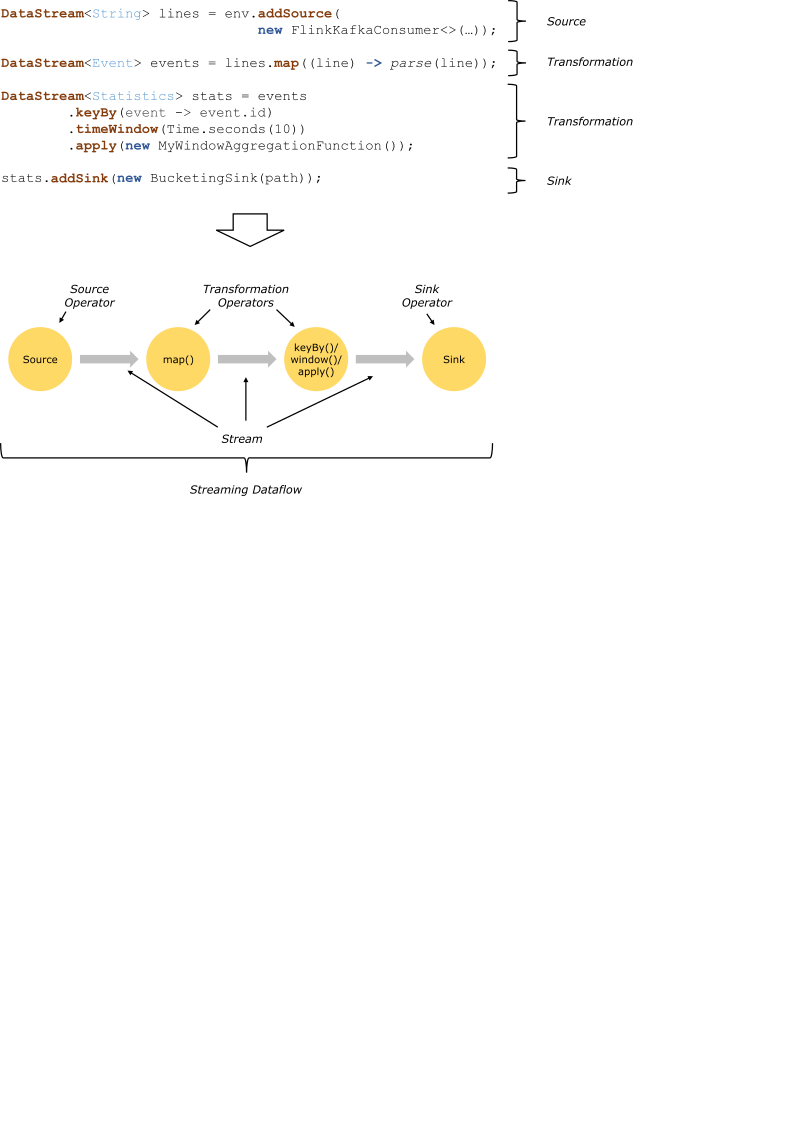
\includegraphics[width=\textwidth]{flink_program_flow.png}
        \caption{Youtube live comments}
        \label{fig:streamexample}
    \end{figure}
\end{frame}


\begin{frame}{Flink Integration}
    \begin{figure}
        \centering
        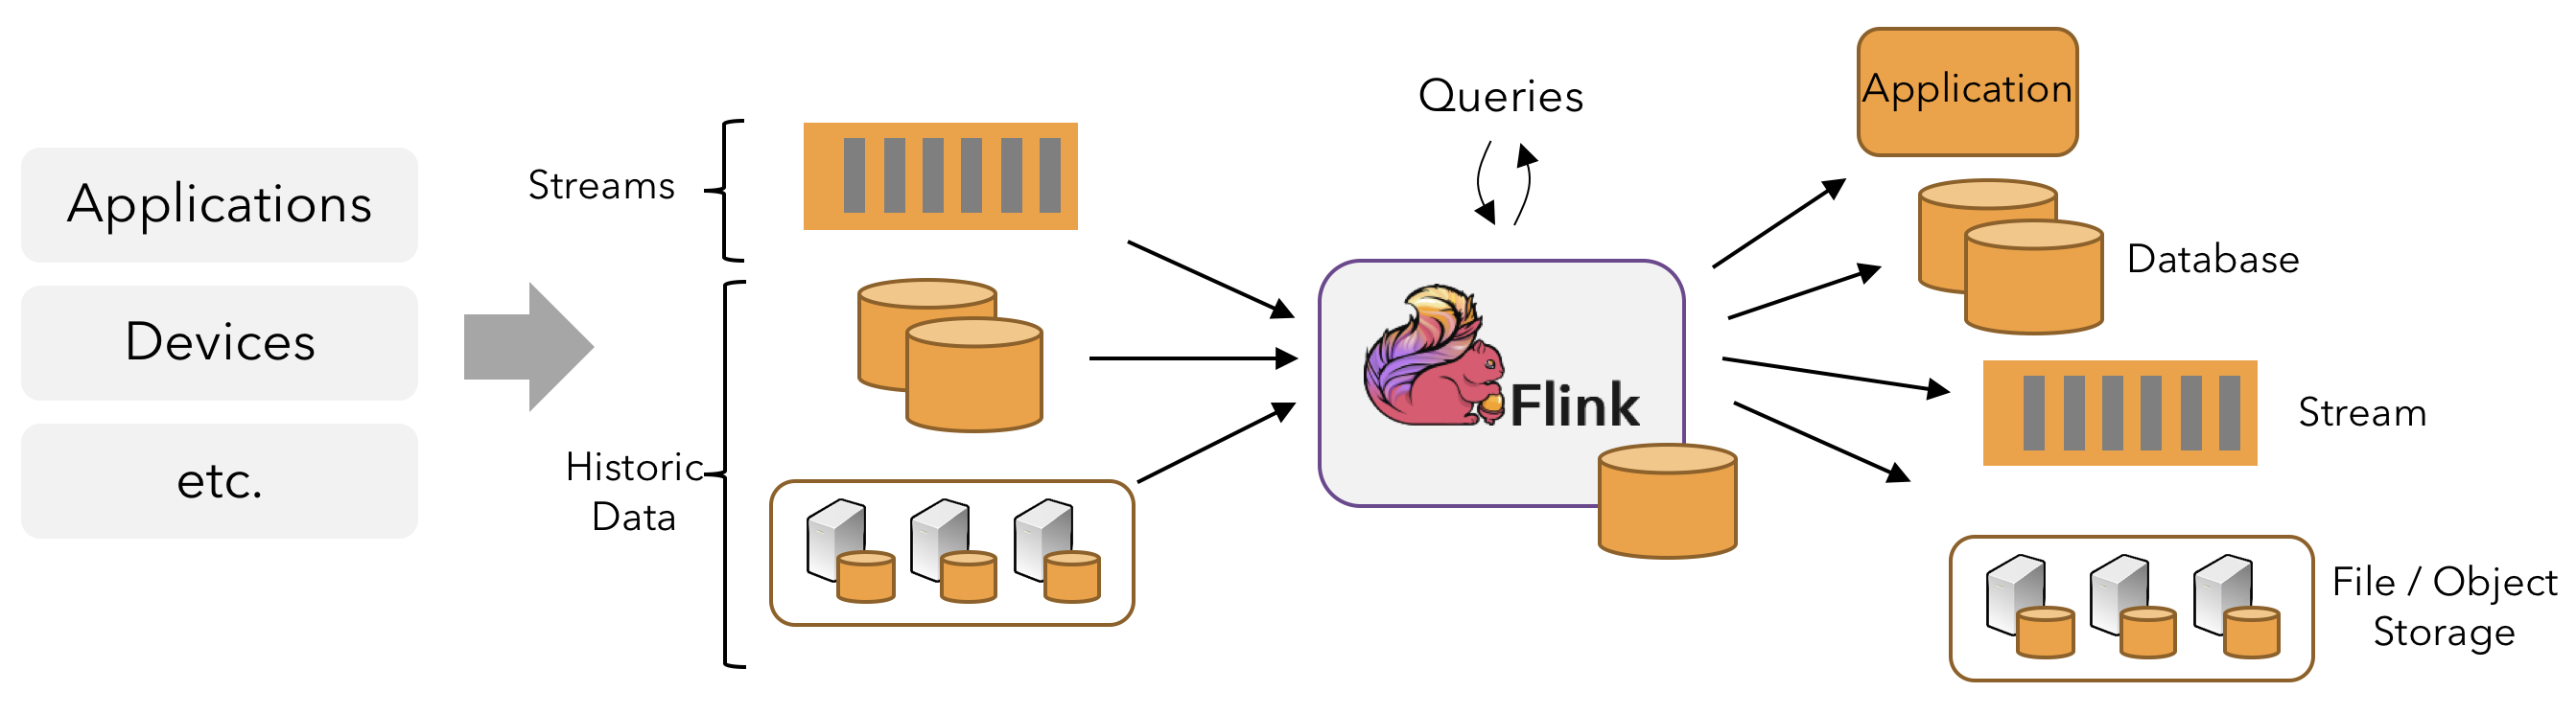
\includegraphics[width=\textwidth]{flink-application-sources-sinks.png}
        \label{fig:streamexample}
    \end{figure}
\end{frame}

\begin{frame}{Stateful processing}
    \begin{figure}
        \centering
        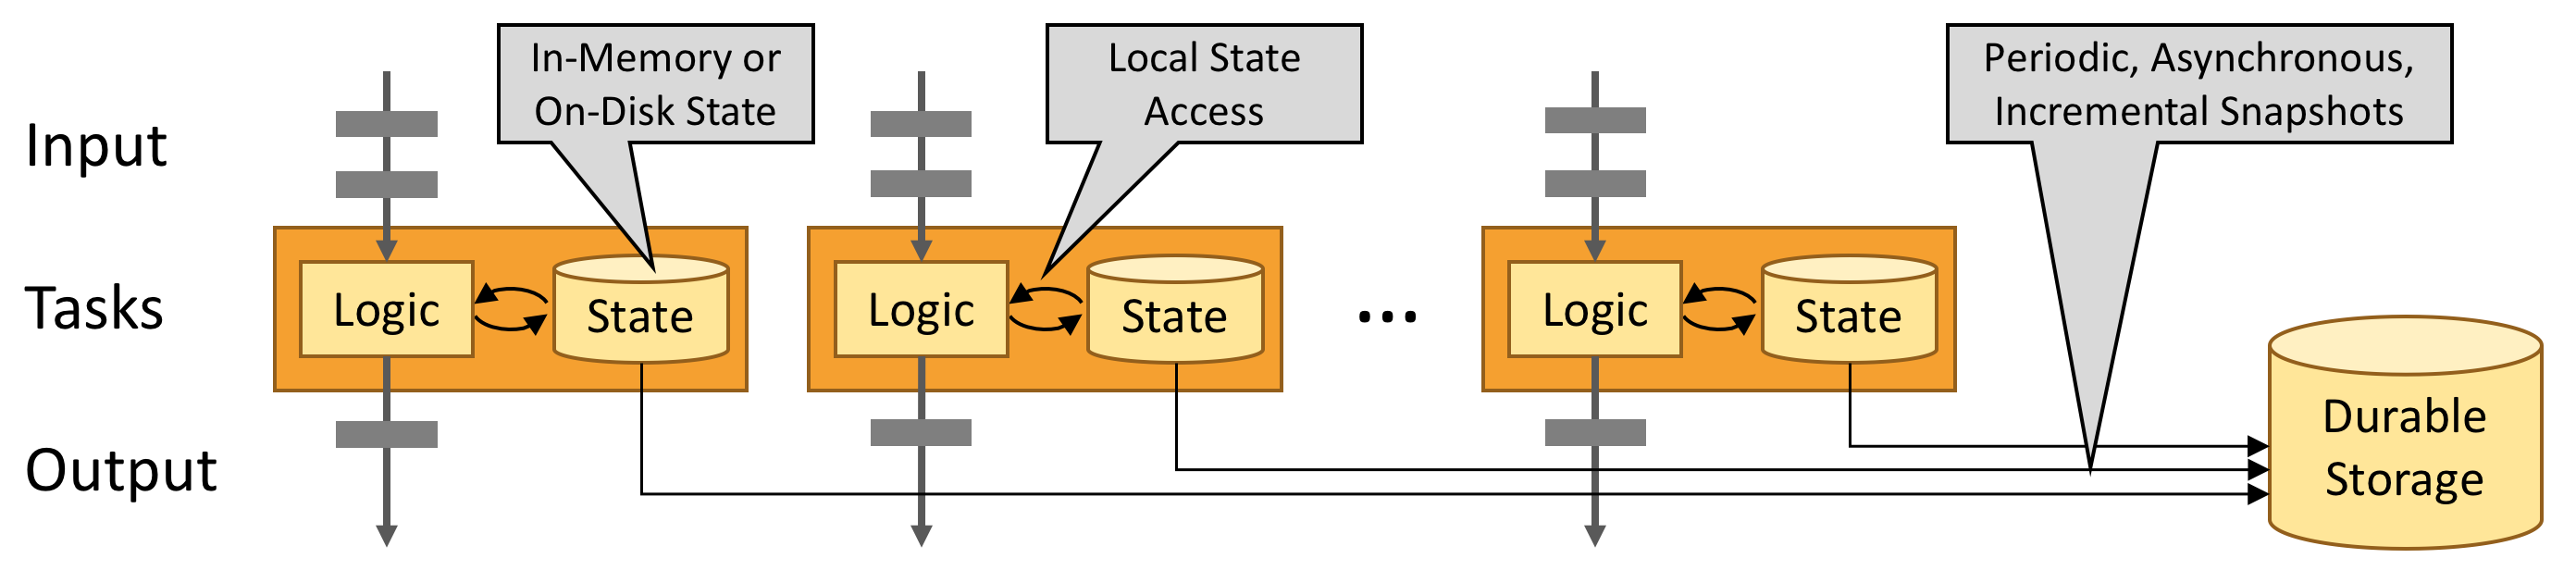
\includegraphics[width=\textwidth]{local-state.png}
        \label{fig:streamexample}
    \end{figure}
\end{frame}
\section{Get Flink running}
\begin{frame}{Installation}
\begin{block}{Starting point}
WE are following the Flink installation page at:
\url{https://ci.apache.org/projects/flink/flink-docs-release-1.11/try-flink/local_installation.html}

\end{block}
\begin{block}{Prerequiste  (for running flink):}
 java 8 or 11
 
 \url{https://www.java.com/en/download/}
 TODO JAVA HOME

Check Java version:
{\tt java -version}

\end{block}
\end{frame}
\begin{frame}{Download Flink binaries}
\url{https://flink.apache.org/downloads.html}
\begin{figure}
        \centering
        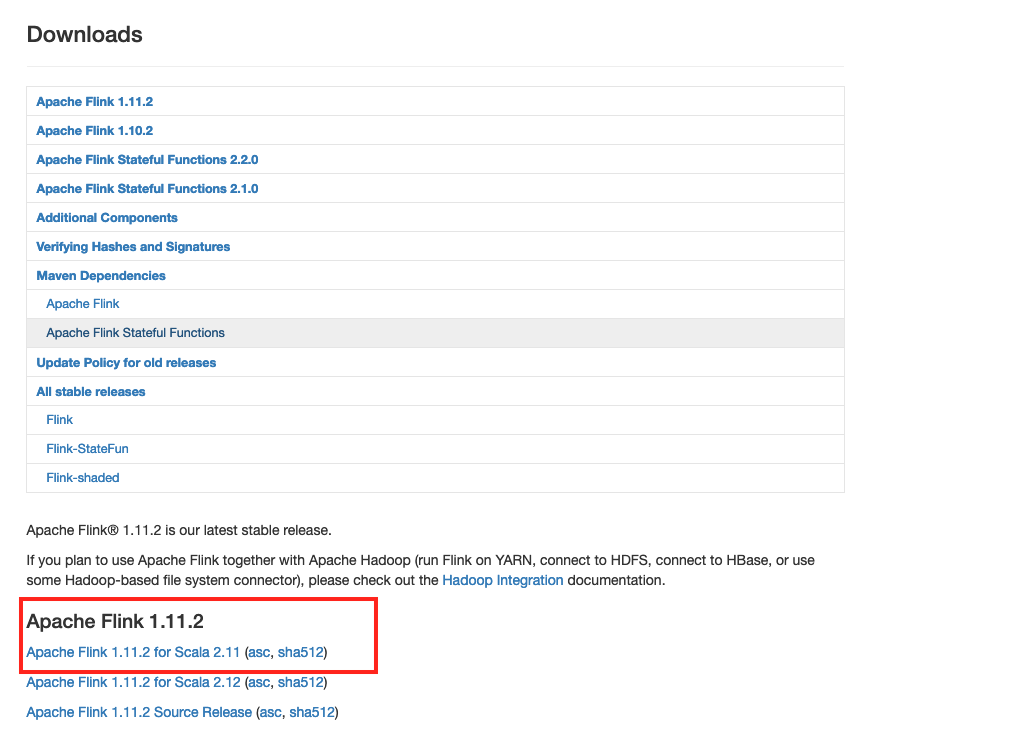
\includegraphics[width=\textwidth]{Flink_download_page.png}
        \label{fig:streamexample}
    \end{figure}

\end{frame}
\begin{frame}{Decompress and start daemon}

\begin{block}{Decompress end enter home directory}
{\tt \$   tar -xzf flink-1.11.2-bin-scala_2.11.tgz\\
\$ cd flink-1.11.2-bin-scala_2.11}
\end{block}
\begin{block}{start daemon}
{\tt    \$ ./bin/start-cluster.sh\\
Starting cluster.\\
Starting standalonesession daemon on host.\\
Starting taskexecutor daemon on host.}
\end{block}
\end{frame}

\begin{frame}{Decompress and start daemon}

\begin{block}{Decompress end enter home directory}
{\tt \$   tar -xzf flink-1.11.2-bin-scala_2.11.tgz\\
\$ cd flink-1.11.2-bin-scala_2.11}
\end{block}
\begin{block}{start daemon}
{\tt    \$ ./bin/start-cluster.sh\\
Starting cluster.\\
Starting standalonesession daemon on host.\\
Starting taskexecutor daemon on host.}
\end{block}
\end{frame}


\begin{frame}{Try flink}

\begin{block}{Run Wordcount example}
{\tt \$ ./bin/flink run examples/streaming/WordCount.jar}
\end{block}
\begin{block}{Check resoults}
{\tt  \$  tail log/flink-*-taskexecutor-*.out}
\end{block}

\begin{block}{Shut down daemon }
{\tt  \$ ./bin/stop-cluster.sh}
\end{block}
\end{frame}


\section{Development}
\begin{frame}{Development tools}

\begin{block}{Prerequiste}
\textbf{JDK} - Java development kit: \url{https://www.oracle.com/java/technologies/javase/javase-jdk8-downloads.html}

\textbf{Apache Maven} - project management tool - for handling dependencies. \url{https://maven.apache.org/install.html} 
\end{block}

\begin{block}{IntelliJ - recommended IDE}
\url{https://www.jetbrains.com/idea/download/}

\end{block}

\begin{block}{Get Flink source (optional for now)}
{\tt  \$ .git clone https://github.com/apache/flink.git}
\end{block}
\end{frame}



\begin{frame}{First project from maven archetype}

following \url{https://ci.apache.org/projects/flink/flink-docs-release-1.11/try-flink/datastream_api.html}

{\tt  \$  mvn archetype:generate \ \\
    -DarchetypeGroupId=org.apache.flink \ \\
    -DarchetypeArtifactId=flink-walkthrough-datastream-java \ \\
    -DarchetypeVersion=1.11.2 \ \\
    -DgroupId=frauddetection \ \\
    -DartifactId=frauddetection \ \\
    -Dversion=0.1 \ \\
    -Dpackage=spendreport \ \\
    -DinteractiveMode=false}
\end{frame}

\begin{frame}{Simple fraud detection}
We consider transactions as fraud when a small transaction is followed by a huge amount, within one minute.

\begin{figure}
        \centering
        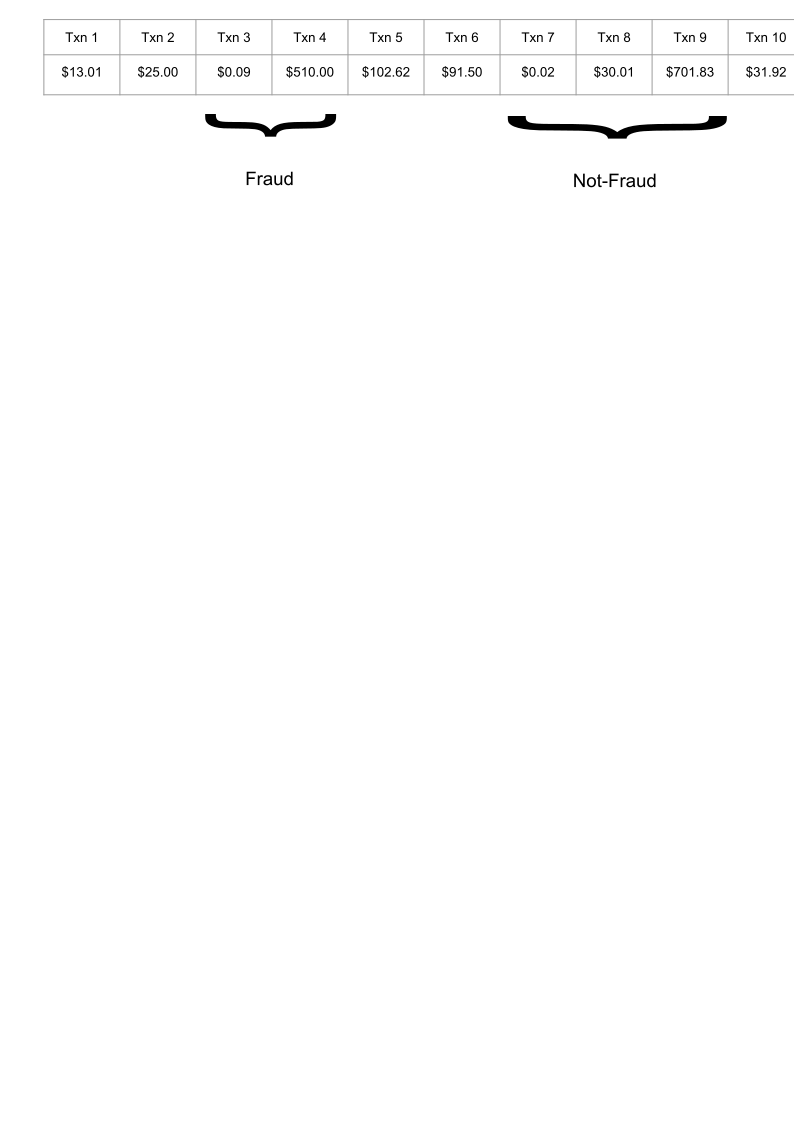
\includegraphics[width=\textwidth]{fraud_detection.png}
        \label{fig:streamexample}
    \end{figure}
\end{frame}

\begin{frame}[fragile]{Pipeline}
\small{
\begin{lstlisting}
public class FraudDetectionJob {
public static void main(String[] args) throws Exception {
    StreamExecutionEnvironment env = 
    StreamExecutionEnvironment.getExecutionEnvironment();

    DataStream<Transaction> transactions = env
        .addSource(new TransactionSource())
        .name("transactions");
    
    DataStream<Alert> alerts = transactions
        .keyBy(Transaction::getAccountId)
        .process(new FraudDetector())
        .name("fraud-detector");

    alerts
        .addSink(new AlertSink())
        .name("send-alerts");

    env.execute("Fraud Detection");
}
}
\end{lstlisting}
}
    
\end{frame}

\begin{frame}[fragile]{Frame Title}



    
 
    

        

        

        

        

\tiny{

\begin{itemize}
    \item {\tt StreamExecutionEnvironment env} context where program is executed - local or remote
    \item {\tt getExecutionEnvironment()} returns EE, if standalone as here a local one
    \item {\tt DataStream<Transaction> transactions} this will be our actual stream of datapoints of type {\tt Transaction}
    \item {\tt env.addSource(new TransactionSource())}  adding the source of the data, where {\tt TransactionSource} is basically an iterator
    \item {\tt transactions.keyBy(Transaction::getAccountId)} give a     partitions the datasream according to \textit{kex} values (the following steps will be executed on streams from data with the same key)
    \item {\tt .process(new FraudDetector())} processing step - applying a transformation/processing step (\tt ProcessFunction),that will emit a new stream 
    \item {\tt ..addSink(new AlertSink())} end of a pipeline, expect a {\tt SinkFunction}
    
    \item {\tt env.execute("...");} triggers the program execution..
\end{itemize}
}

%}    
\end{frame}

\begin{frame}{State Variables for processing}
%TODO how does keyby works?? already  a hashing??

{\tt  ValueState<T>} 

When a stream has been partitioned based on a given attribute({\tt keyby(..)}) it is possible to add a state, that will be maintained for each keys.

It it a wrapper class that can hold any type, its methods are :
\begin{itemize}
    \item {\tt .value()} to get the actual value it holds
    \item {\tt .update()} to change the actual value it holds
    \item {\tt .clear()} to remove the actual value it holds(\texttt{=null})
    
\end{itemize}
Creation: ask the \texttt{ExecutionEnvironment}:
\small{
\texttt{ValueStateDescriptor<Boolean> flagDescriptor \\
= new ValueStateDescriptor<>("flag",Types.BOOLEAN);\\
flagState = getRuntimeContext().getState(flagDescriptor);}

}
    
\end{frame}

\begin{frame}[fragile]{Processing time timers}

Search for patterns within a time interval
\small{
\begin{lstlisting}
ValueStateDescriptor<Long> timerDescriptor 
   = new ValueStateDescriptor<>("timer-state", Types.LONG);
timerState = getRuntimeContext().getState(timerDescriptor);
\end{lstlisting}

Intuition: when a data point  triggers the observation of the pattern, we set up a state variable(as before) and a timer:
\begin{lstlisting}
long timer = context.timerService().currentProcessingTime()
    + ONE_MINUTE;
context.timerService().registerProcessingTimeTimer(timer);
    timerState.update(timer);
\end{lstlisting}
and add an event listener for the case when the time is up:
\begin{lstlisting}
@Override
public void onTimer(long timestamp, OnTimerContext ctx,
        Collector<Alert> out) {
    // remove flag after 1 minute
    timerState.clear();
    flagState.clear();
}
\end{lstlisting}
}


\end{frame}


\begin{frame}[fragile]{Create state}
\small{
State variables should be created before the process starts, that is in the inherited \texttt{open} function of process functions.

\begin{lstlisting}
public class FraudDetector extends KeyedProcessFunction<Long,
Transaction, Alert> {
    private transient ValueState<Long> timerState;
    ...
    @Override
    public void open(Configuration parameters) {
        ValueStateDescriptor<Long> timerDescriptor 
        = new ValueStateDescriptor<>(
                "timer-state",
                Types.LONG);
        timerState = getRuntimeContext()
         .getState(timerDescriptor);
    }
    timerState = getRuntimeContext()
        .getState(timerDescriptor);
}    
\end{lstlisting}
}
\end{frame}
%==========

\begin{frame}[fragile]{Remove timer service}

When we do not need it anymore, we have to remove the timer service from the environment, then set the value of the reference to \texttt{null}:
\begin{lstlisting}
Long timer = timerState.value();
ctx.timerService().deleteProcessingTimeTimer(timer);
timerState.clear();
\end{lstlisting}
\end{frame}
%==========

\begin{frame}{Hash and Bloom filter}
hashcode \url{https://www.javamex.com/tutorials/collections/hash_codes_advanced_duplicate_elimination.shtml}
   \url{https://www.javamex.com/tutorials/collections/bloom_filter.shtml}
\end{frame}




\begin{frame}[allowframebreaks]{Bibliography}
\fontsize{8pt}{7.2}\selectfont
\bibliographystyle{apalike}
\bibliography{./TKDE}
\end{frame}
\end{document}